\documentclass[11pt]{article}

\usepackage{graphicx}

% Enable references to labels in the notes
\usepackage{xr-hyper}
\externaldocument{p328_notes}
\usepackage{hyperref}

% Sans fonts
\usepackage{sfmath}
\renewcommand{\familydefault}{\sfdefault}

\newcommand{\COURSE}{PHYS328W}
\newcommand{\LABNUM}{6}
\newcommand{\TITLE}{Transistor Behavior}
\markright{\COURSE~Lab \LABNUM\ : \TITLE}

\setlength{\textwidth} {6.5 true in}
\setlength{\textheight}{9 true in}
\setlength{\hoffset}   {-0.75 true in}
\setlength{\voffset}   {-0.75 true in}
\setlength{\parindent} {12 pt}
\pagestyle{myheadings}

\begin{document}

\thispagestyle{empty}

\section*{\COURSE\ Lab \LABNUM\ : \TITLE}

This assignment relies on Section~\ref{sec:transistors} of the notes.

\subsection*{Experiments}

\begin{figure}[ht]
  \begin{center}
    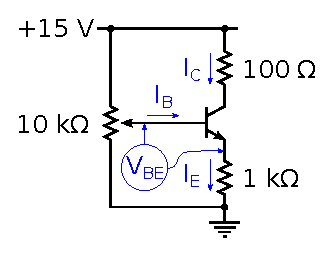
\includegraphics{ebersmollcircuit.eps}
    \caption{Schematic of the circuit you will use in lab to
      test the Ebers-Moll equation in the active region of an NPN
      BJT.}
    \label{fig:ebersmollcircuitlab}
  \end{center}
\end{figure}

\begin{enumerate}
\item Make sure the power switch on your prototyping board is off.

\item Find 100~$\Omega$ and 1~k$\Omega$ resistors, a 10~k$\Omega$ pot,
  and a \texttt{2N3904} NPN transistor.

\item Measure the resistances of the 100~$\Omega$ and 1~k$\Omega$
  resistors with a DMM.
  
\item Construct the circuit shown in
  Figure~\ref{fig:ebersmollcircuitlab}. 

\item Use the DMM to confirm which direction to turn the pot to
  increase/decrease the resistance. This depends on how the pot is
  oriented on the prototyping board relative to the rest of the
  circuit.
  
\item Turn the pot all the way down so that the transistor will start
  in the ``off'' state, and turn on the power to your prototyping 
  board.

\item Turn on the prototyping board, and set the positive variable
  supply voltage to 15~V.

\item While monitoring the voltage drop across the 100~$\Omega$
  collector resistor, slowly turn up the pot, collecting several sets
  of $I_C$, $I_E$, and $V_{BE}$ measurements in the range over which
  $I_C$ and $I_E$ vary.
  \begin{itemize}
  \item Use Ohm's law to determine $I_C$ and $I_E$ from the measured
    voltage drops across the collector and emitter resistors and their
    measured resistances.
  \item Note that $V_{BE}$ is \emph{not} the potential difference
    between the base and ground. The DMM probe placement is
    illustrated in Figure~\ref{fig:ebersmollcircuitlab}.
  \item Map the ``off'' and active states of the transistor. 
  \end{itemize}
  \emph{If the emitter potential is held above that of the base, the
    transistor will no longer be able to operate as advertised. You
    should see this happen very close to the top of the range of the
    pot.}

\item Plot $\ln(I_C)$ vs. $V_{BE}$, compare it with the behavior
  predicted by the Ebers-Moll equation (Equation~\ref{eq:ebersmoll} in
  the notes).

\item If the Ebers-Moll equation appears to be a reasonable model,
  determine values of the leakage current $I_o$ and the temperature by
  fitting a line to the portion of your $\ln(I_C)$ vs. $V_{BE}$ graph
  in the active region. 

\item In your spreadsheet, calculate the base current $I_B = I_E -
  I_C$ at each value of $V_{BE}$.
  
\item Determine $h_{FE}$ values from your $I_B$ and $I_C$ values, and
  make a graph of $h_{FE}$ vs. $V_{BE}$.
\end{enumerate}

\subsection*{Simulations}

\emph{Do not expect more than qualitative agreement between simulation
and measurement. There is variation among transistors of the same
make/model, so the PSpice model parameters are only representative. It
is enlightening to see how much variation we see between the transistors
studied by different lab groups.}

\begin{enumerate}
\item Construct the circuit shown in
  Figure~\ref{fig:ebersmollcircuitlab}. For the transistor, click on
  \texttt{Place -> Part ...}, type Q2N3904 into the search bar, and
  select \texttt{Q2N3904/BIPOLAR}.

  If the part does not show up in the \texttt{Part List} panel, you
  need to add a library. Click the \includegraphics{OrCAD_AddLib.png}
  button in the \texttt{Libraries} panel, select the file
  \texttt{bipolar.olb}, and click \texttt{Open}. Then, select the
  \texttt{BIPOLAR} library in the \texttt{Libraries} panel, and try
  searching for \texttt{Q2N3904/BIPOLAR} again.
  
\item Set up a parameter you can use in a DC sweep analysis to vary
  the pot.
  \begin{itemize}
    \item Click on \texttt{Place -> Part ...}, enter \texttt{PARAM} into
      the search bar, and place it anywhere on your schematic.

      If the \texttt{PARAM} part does not show up in the
      \texttt{Part List} panel, you need to add a library. Click the
      \includegraphics{OrCAD_AddLib.png} button in the
      \texttt{Libraries} panel, select the file \texttt{special.olb}, 
      and click \texttt{Open}. Then, select  the \texttt{SPECIAL}
      library in the \texttt{Libraries} panel, and try searching for
      \texttt{PARAM} again. 
      
    \item Double-click on \texttt{PARAMETERS:} in the schematic, and
      click on the \texttt{New Property ...} button. Name the property
      psetvariable, and set its value to 0.5. Check the
      \texttt{Display} box, and select \texttt{Name and Value} under
      \texttt{Display Format}.
    \item Change the value of the \texttt{SET} parameter of the pot to
      \verb+{psetvariable}+ (the curly braces are important).
  \end{itemize}

\item Create a new simulation profile, and set the \texttt{Analysis
  Type} to \texttt{DC Sweep}. Select \texttt{Global parameter} under
  \texttt{Sweep Variable}, and set the parameter name to
  \texttt{psetvariable}. Select \texttt{Linear} under \texttt{Sweep
    Type}, and set \texttt{Start Value}, \texttt{End Value}, and
  \texttt{Increment} to 0, 1, and 0.01.

\item In the schematic, place a current probe to measure the collector
  current $I_C$.

\item Make note of the names of the points at which you measure
  $V_{BE}$ by hovering the pointer over them.

\item Run the simulation.

\item In the \texttt{PSpice A/D Lite} window, you will find a plot of
  the current vs. the pot setting. Instead, set up a plot of
  $\ln(I_C)$ vs. $V_{BE}$.
  \begin{enumerate}
  \item Double-click on the horizontal axis, and click on the
    \texttt{Axis Variable ...} button. In the \texttt{Trace
      Expression:} entry box, enter the base voltage minus the emitter
    voltage, using the names you found in the schematic.
  \item Right-click and select \texttt{Add Trace}. In the \texttt{Trace
      Expression:} entry box, enter \texttt{LOG(ABS(I(R2)))}. (If the
    current displayed automatically is something other than
    \texttt{I(R2)}, use that in the expression instead.)
  \item So that you don't lose this setup the next time you run the
    simulation, edit the simulation profile, and select the
    \texttt{Last Plot} radio button on the \texttt{Probe Window} tab.
  \item Right click on the trace, and select \texttt{Copy to
    Clipboard}. Paste the data into your spreadsheet, and add it to
    your $\ln(I_c)$ vs. $V_{BE}$ graph.
  \end{enumerate}
\end{enumerate}

\subsection*{Products}

Upload to Canvas a brief \LaTeX\ report in which you comment on ...
\begin{itemize}
  \item the degree to which your measurements in the active region are
    compatible with the Ebers-Moll equation,
  \item the dependence (if any) of the current gain $h_{FE}$ on
    $V_{BE}$, and
  \item the level of agreement between your simulation and
    measurements.
\end{itemize}
Include as figures your graphs of $\ln(I_C)$ vs. $V_{BE}$ and $h_{FE}$
vs. $V_{BE}$. Report the values of $I_o$ and $T$ you determined for
your transistor.

\end{document}
